In the past year, the work by \cite{hu2017toward} and \cite{ficler2017controlling} both expounded the applicability of attribute-conditioned generated to linguistic style transfer tasks. Both of these methods, as opposed to the historical used paraphrasing methods \citep{xu2012paraphrasing}, utilized neural network models \citep{lecun2015deep} to learn the style transfer function.

Further work presented by \cite{shen2017style} and \cite{fu2017style} utilize the idea of removing attribute information from latent representations using adversarial learning. In this section we discuss some of the prominent work done in this area.

\section{Disentangling Factors of Variation}

\cite{mathieu2016disentangling} proposed the idea of a generative model that learns to separate the factors of variation in the learned representations by splitting the latent space into two codes - one that is relevant to solving a specialized tasks, and one that is not relevant to the specialized task.

They use a variational autoencoder to learn the generative model, and utilize adversarial training to disentangle the latent space of specific attributes. In their evaluations, they utilize image data-sets like MNIST \citep{lecun2010mnist}, NORB \citep{lecun2004learning}, Sprites \citep{reed2015deep} and Extended-YaleB \citep{georghiades2001few}.

Handwriting style, body type, hair, position, illumination etc. are some of the chosen attributes to disentangle from the latent space. This disentanglement is done by training a discriminator, following \cite{goodfellow2014generative} to provide a negative training signal to the generative model if it is able to discriminate training samples based on the given attribute. Once the model is converged and they are able to produce representations devoid of the chosen style or attribute, they can generate new instances of data, conditioned on known representations, but changing the controlled attribute, to product novel samples.


\section{Information Maximizing Generative Adversarial Nets}

InfoGAN \citep{chen2016infogan} is another work that attempts increasing the interpretability of latent representation by utilizing additional regularizations on the latent space to maximize the information retention of attributes in subsets of the overall latent space.

The authors present a modification to the GAN objective \citep{goodfellow2014generative} to encourage the learning of interpretable representations. This is done by maximizing the
mutual information between a fixed small subset of the GAN's noise variables and the observations. This approach attempts to learn a disentangled latent representation unsupervisedly. In addition to the regular noise variables that a GAN generates novel samples from, the authors use additional categorical and continuous variables under certain sampling constraints. For examples on the MNIST data-set \citep{lecun2010mnist}, the authors use a categorical latent variable of size size, with the probability of sampling each of those variables discretely as 0.1, to represent the 10 distinct digits (labels) present in the MNIST data-set. In addition, they sample two continuous variables sampled from $Unif(-1, 1)$.

In the vanilla formulation of the GAN, the decoder might well chose to ignore these additional latent variables provided by minimizing the magnitude of the parameters learned between the additional latent variable and a generated sample. To avoid this, the authors propose an information maximization objective as an auxillary training objective to the GAN objective.

Using this approach, the authors are able to generate MNIST digits in various handwriting styles by changing the continuous variables, and change the numerical value represented in the generated image by changing the categorical variable, as shown in Figure \ref{fig:images/infogan-digits}. Here $c_1$ represents the categorical variable discussed above and $c_2, c_3$ represent continuous variables.

\begin{figure}[ht]
	\centering
	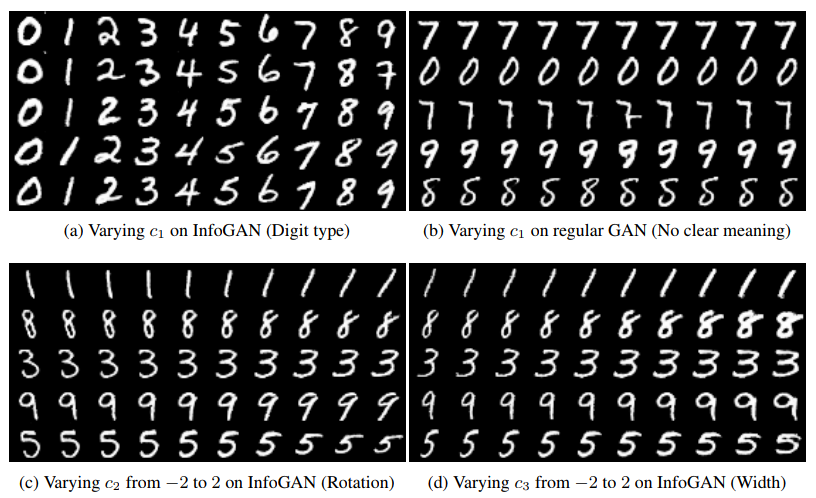
\includegraphics[width=\textwidth]{images/infogan-digits}
	\imgsrc{\cite{chen2016infogan}}
	\caption{\label{fig:images/infogan-digits} InfoGAN: Tweaking Latent Variables}
\end{figure}

However, this method does not provide a method of explicitly controlling the nature of the sampled data. Samples need to be generated first to understand which features have been represented in the additional latent variables.


\section{Controlled Generation of Text}

\cite{hu2017toward} use a variational autoencoder trained with the reconstruction objective and a KL-divergence minimization objective on the latent space with respect to a prior $p(z)$, as described in the original variational auto-encoding paper by \cite{kingma2013auto}. In addition to the reconstruction objective, the authors use additional discriminative training signals to adapt the desired attributes of the generated text. These training signals need to be propagated back to the encoder.

$x$ is the source corpus and the encoder is parameterized to generate a latent code $z$, which is a variational latent space that resembles a Gaussian prior. (This is enforced by a KL-divergence loss). The structured code $c$ is a known label of the text (discrete or continuous). The decoder generator produces the output corpus $\hat{x}$ conditioned on $(z, c)$. It uses greedy decoding, which predicts the word with maximal probability at each step \citep{langlais2007greedy}.

A classifier/regressor discriminator predicts the structured code of the output corpus $\hat{x}$ to ensure that it is the same as the one the generator was conditioned on i.e. $G(z, c)$. The discriminator is pre-trained.

Each decoder step in $\hat{x}$ is predicted using a softmax function scaled by a temperature $\tau$. Higher temperatures flatten the softmax distribution for each word prediction and increase word diversity. Conversely, setting $\tau = 0$ will resemble a discrete probability distribution over the corpus vocabulary. For their experiments, the authors gradually anneal $\tau \rightarrow 0$

The authors describe the following objectives to train their model:

\subsection{Variational Autoencoder}

A reconstruction loss that ensures that the generated sentence $\hat{x}$ is the same as the original sentence $x$. This is equivalent to minimizing the negative log-likelihood of generating $\hat{x}$. This is shown in Equation \ref{eqn:tcg-rec}
\begin{eqnarray} \label{eqn:tcg-rec}
	\mathcal{L}_{VAE}(\theta_G, \theta_E; x) &=& \nonumber
	- \mathbb{E}_{q_E(z|x)q_D(c|x)}[log p_G(x|z,c)] \\ & &
	+ KL(q_E(z|x)||p(z))
\end{eqnarray}


\subsection{Style Discriminator}

A discriminator validates if the predicted class/value for $\hat{x}$ is the same as the corresponding class/label for $x$. This is a cross-entropy loss over the probability distribution of the labels. This discriminator loss can be further subdivided into 2 terms, one that maximizes the log likelihood of predicting the correct class as in Equation \ref{eqn:tcg-disc-class}, and one that minimizes the empirically observed Shannon entropy of the predicted distribution, thereby incentivizing confident predictions, as in Equation \ref{eqn:tcg-disc-ent}.
\begin{equation} \label{eqn:tcg-disc-class}
	\mathcal{L}_s(\theta_D) = - \mathbb{E}_{X_L}[log q_D(c_L|x_L)]
\end{equation}
\begin{equation} \label{eqn:tcg-disc-ent}
	\mathcal{L}_u(\theta_D) = - \mathbb{E}_{p_G(\hat{x}|z,c)p(z)p(c)}
	[log q_D(c|\hat{x}) + \beta \mathcal{H}(q_D(c'|\hat{x}))]
\end{equation}


\subsection{Content Discriminator}

The encoder from loss equation \ref{eqn:tcg-rec}, is used to regenerate the latent distribution $z$ devoid of the structured code from the output distribution $\hat{x}$. The authors call this an \textbf{independence constraint}, in that regardless of the structured code $c$ that is currently present in either $x$ or $\hat{x}$, processing either through the generator should produce a consistent $z$. This allows the encoder to encode only latent factors that are independent of the structured code. This is shown in Equation \ref{eqn:tcg-ind-con}.
\begin{equation} \label{eqn:tcg-ind-con}
	\mathcal{L}_{attr, z}(\theta_G) = - \mathbb{E}_{p(z)p(c)}
	[log q_E(z|\tilde{G_{\tau}}(z,c))]
\end{equation}


They maximize the expected log likelihood of predicting the correct distribution of the structured code $c$ given the labelled examples $X_L$. This happens before the generator model training. They also maximize the expected log likelihood of predicting the correct distribution of the structured code $c$ given the generated sentences $\hat{x}$. Also minimize the empirically observed Shannon entropy of the observed discriminator prediction $q_D(c'|\hat{x})$, which reduces uncertainty and increases confidence of the structured code prediction. A wake-sleep algorithm \citep{hinton1995wake} is used to alternatively train the generator and discriminator.

The model was applied only to short sentences with length $<15$ words and the encoder-decoder setup is implemented using single layer LSTMs and the discriminator is implemented using a convolutional neural network (CNN). The KL loss weight is annealed from 0 to 1 during training.


\section{Aligned and Cross-Aligned Autoencoders}

\cite{shen2017style} aim to perform style transfer on language using non-parallel corpora by separating content from style. They re-align the latent spaces to perform three tasks: sentiment modification, decipherment of word-substitution ciphers, and recovery of word order. Their method involves learning an encoder that takes a sentence and its original style label as input, and maps it to a content representation devoid of style. This representation is then decoded by a decoder whose input is this encoded representation and the target style label.

There are two non-parallel corpora $X_1 = {x_1^{(1)} ... x_1^{(n)}}$, drawn from the prior $p(x_1|y_1)$ and $X_2 = {x_2^{(1)} ... x_2^{(n)}}$, drawn from the prior $p(x_2|y_2)$. The objective is to estimate the style transferred distributions $p(x_1|x_2;y_1,y2)$ and $p(x_2|x_1;y_1,y2)$.

The authors propose a constraint that $x_1$ and $x_2$'s marginal distributions can only be recovered if for any different styles $y, y' \in Y$, distributions $p(x|y)$ and $p(x|y')$ are different, which is a fair assumption to make because if $p(x|y)$ = $p(x|y')$, then the style changes would be indiscernible.

They also prove that if the content $z$ is sampled from a centered isotropic distribution, the styles cannot be recovered from $x$, but in the case of $z$ being a more complex distribution like a Gaussian mixture, then the affine transformation that converts $y, z$ into $x$ can be recovered.

The reconstruction loss is the same as the one used by a variation autoencoder for its reconstruction objective, as shown in Equation \ref{eqn:stca-rec}.
\begin{eqnarray} \label{eqn:stca-rec}
	\mathcal{L}(\theta_E,\theta_G)
	&=& \mathbb{E}_{x_1 \sim X_1}[-\log p_G(x_1|y_1,E(x_1, y_1))] \nonumber \\
	& & + \mathbb{E}_{x_2 \sim X_2}[-\log p_G(x_2|y_2,E(x_2, y_2))]
\end{eqnarray}

\subsection{Aligned Autoencoder}

The authors propose aligning the distributions $P_E(z|x_1)$ and $P_E(z|x_2)$ where $E$ is the encoder function. This is done by training an adversarial discriminator to distinguish between the two distributions.

The adversarial objective is expressed as below where $D(\cdot)$ predicts 0 if it predicts the source distribution to be $X_1$ and 1 if it predicts the source distribution to be $X_2$
\begin{eqnarray} \label{eqn:stca-align-adv}
	\mathcal{L}_{adv}(\theta_E,\theta_D)
	&=& \mathbb{E}_{x_1 \sim X_1}[-\log D(E(x_1,y_1))] \nonumber \\
	& & + \mathbb{E}_{x_2 \sim X_2}[-\log(1 - D(E(x_2,y_2)))]
\end{eqnarray}

The overall optimization objective combining equations \ref{eqn:stca-rec} and \ref{eqn:stca-align-adv} can be written as
\begin{equation}
	\mathcal{L} = \operatorname*{min}_{E,G} \operatorname*{max}_{D} \mathcal{L} - \lambda \mathcal{L}_{adv}
\end{equation}
where $\lambda$ is a balancing weight for the adversarial term.

\subsection{Cross-aligned Autoencoder}

This is similar to the aligned autoencoder approach, but instead of trying to align $P_E(z|x_1)$ and $P_E(z|x_2)$ using an adversarial discriminator, two distinct adversarial discriminators are used to align a sequence of real and transferred generator hidden states. i.e. $D_1$ is used to align the distributions $G(y_1, z_1)$ and $G(y_1, z_2)$. Similarly, $D_2$ is used to align the distributions $G(y_2, z_2)$ and $G(y_2, z_1)$. These discriminators are trained with the objective of being unable to identify the content distributions $P(z_1)$ and $P(z_2)$

Professor-forcing is used to train both of these discriminators. Professor forcing uses a discriminator to distinguish if the decoder hidden states are a result of training-time teacher forcing or test time scheduled sampling \citep{lamb2016professor}. This is a generalized version of simply using a final encoder state, as was the case in the Aligned Autoencoder solution.

The overall optimization objective combining equation \ref{eqn:stca-rec} and two discriminator variants of equation \ref{eqn:stca-align-adv} can be written as:
\begin{equation}
	\mathcal{L} = \operatorname*{min}_{E,G} \operatorname*{max}_{D} \mathcal{L} - \lambda (\mathcal{L}_{adv_1} + \mathcal{L}_{adv_2})
\end{equation}

As opposed to the simple feed-forward classifier used in the aligned autoencoder, the cross-aligned autoencoder uses convolutional nets for text classification. They use Yelp reviews as the data set with rating $>3$ as positive and rating $<3$ as negative examples. Reviews with a sentence count $>10$ and sentences with a word count $>10$ are filtered out. The vocabulary size used is $10K$. Style transfer is evaluated using a pre-trained classifier. Language fluency and content preservation was evaluated using human assessments.

\section{Style Embedding Autoencoder}

\cite{fu2017style} employ two distinct models to perform style transfer
\begin{itemize}
	\item A \textbf{multi-decoder model} that use the distinct decoders to produce text in different styles. This implicitly means that the number of decoders that need to be trained scales with the number of distinct label values to train.
	\item A \textbf{style-embedding model} with a single decoder that generate text in different styles. This method utilizes a separate style embedding matrix, of size $n * m$ where $n$ is the number of distinct label values and $m$ is an arbitrarily chosen embedding size.
\end{itemize}

In contrast with the previous models described, this work uses a deterministic autoencoder in lieu of a variational autoencoder. For our purposes, we focus on the style-embedding model, since it requires explicit disentanglement and uses fewer model parameters for each label addition, compared to the multi-decoder model.

The training objectives used for this model include the reconstruction objective for the autoencoder, the style label discriminative objective for a classifier on the latent space, and the adversarial loss propagated back to the autoencoder from the representation learned in the content space.

The autoencoder is trained to product only the salient features that represent the content of the sentences i.e. the content space, and the style embedding vector is trained via back-propagation of the reconstruction loss.

The reconstruction loss is the same as that of a standard deterministic autoencoder.
\begin{equation}
	\mathcal{L}_{seq2seq} = -\sum_{i=1}^M \log P(\hat{x}_i|x_i;\theta_e;\theta_d)
\end{equation}
where $M$ is the number of training examples and $\theta_e$ and $\theta_d$ are the encoder and decoder parameters respectively.

A discriminative classifier is trained on the latent content space learned by the autoencoder, to distinguish between the different possible styles.
\begin{equation}
	\mathcal{L}_{disc} = -\sum_{i=1}^M \log P(l_i|Encoder(x_i;\theta_e);\theta_c)
\end{equation}
where $M$ is the number of training examples and $\theta_e$ and $\theta_c$ are the encoder and discriminative classifier parameters respectively.

An adversarial objective is applied to the content representation. This objective aims to maximize entropy of the predicted label from the content representation by minimizing the following objective:
\begin{equation}
	\mathcal{L}_{adv} = -\sum_{i=1}^M\sum_{j=1}^N \mathcal{H}(P(j|Encoder(x_i; \theta_e); \theta_c))
\end{equation}
where $M$ is the size of the training data and $N$ is the number of distinct styles. Using this adversarial entropy objective, the encoder is penalized and therefore trained to produce a latent content representation which is independent of style.

Similar to the persona-based neural conversation model \citep{li2016persona}, a style embedding is learned for each different style. The conditional generation is done using recurrent neural networks with the inputs being the recurrent networks current state, and the style embedding to apply.

The style embeddings matrix is not directly parameterized by the encoder, but the learning algorithm propagates changes based on how well it combines with the content representation to reconstruct the original text.

The methods are evaluated in the following manner:
\begin{itemize}
	\item Transfer strength is evaluated using a simple classifier
	\item Content preservation is evaluated by computing the cosine distance between the original and the generated text embeddings.
\end{itemize}


Several other works have also been published in this domain recently including using cyclical translation to strip style as a pre-processing step, followed by a multi-decoder model to generate style-transferred sentences \citep{prabhumoye2018style},

